\section{Regression}

Regression analysis is a fundamental statistical technique used to model and understand the relationship between a response variable \( Y \) and one or more explanatory variables \( X_1, X_2, \ldots, X_p \). The goal is to estimate a function \( f(X) \) that captures the systematic relationship between \( X \) and \( Y \), while accounting for random variation (error).

\subsection{Additive Error Models}

We often assume an additive model of the form:
\[
Y = f(X) + \varepsilon,
\]
where \( \varepsilon \) is a random error term with
\[
\mathbb{E}[\varepsilon] = 0, \quad \text{and} \quad \text{Var}(\varepsilon) = \sigma^2.
\]
The term \( \varepsilon \) captures the \textbf{irreducible error}—random variation that cannot be explained by the model, even with perfect knowledge of \( f \).

A common goal is to estimate the \textbf{regression function}:
\[
f(X) = \mathbb{E}[Y|X].
\]
This represents the expected value of \( Y \) for a given value of \( X \).

\subsection{Estimating \( f(X) \)}

Given a set of training data \((x_1, y_1), \ldots, (x_n, y_n)\), we want to construct an estimate \(\hat{f}(X)\) that minimizes the expected prediction error:
\[
\mathbb{E}\left[(Y - \hat{f}(X))^2\right].
\]

\subsubsection{K-Nearest Neighbour (KNN) Regression}

A simple non-parametric estimator is the \textbf{K-nearest neighbours (KNN)} regression:
\[
\hat{f}(x_0) = \frac{1}{K} \sum_{x_i \in \mathcal{N}_K(x_0)} y_i,
\]
where \(\mathcal{N}_K(x_0)\) is the set of the \(K\) closest training points to \(x_0\).

\paragraph{Example:}
For example, to predict \( f(4) \), we take the average of the \(Y_i\) values for the \(K\) data points whose \(X_i\) values are closest to \(4\):
\[
\hat{f}(4) = \text{avg}\{Y_i : X_i \in \mathcal{N}_K(4)\}.
\]

\paragraph{Advantages and Limitations:}
\begin{itemize}
    \item Performs well when the number of predictors \(p\) is small and sample size \(n\) is large.
    \item Performs poorly when \(p\) is large due to the \textbf{curse of dimensionality}—as \(p\) increases, points become sparse, and distances between them lose meaning.
\end{itemize}

\begin{center}
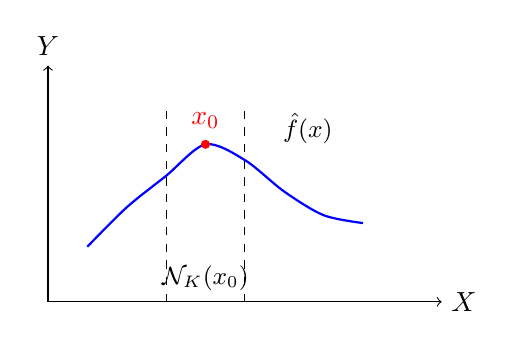
\begin{tikzpicture}[scale=1.0]
\draw[->] (0,0) -- (5,0) node[right] {$X$};
\draw[->] (0,0) -- (0,3) node[above] {$Y$};
\draw[blue, thick] plot[smooth] coordinates {(0.5,0.7) (1,1.2) (1.5,1.6) (2,2) (2.5,1.8) (3,1.4) (3.5,1.1) (4,1)};
\node at (3.3,2.2) {\small $\hat{f}(x)$};
\draw[red, fill=red] (2,2) circle (0.05);
\node[red] at (2,2.3) {$x_0$};
\draw[dashed] (1.5,0) -- (1.5,2.5);
\draw[dashed] (2.5,0) -- (2.5,2.5);
\node at (2,0.3) {\small $\mathcal{N}_K(x_0)$};
\end{tikzpicture}

\textit{Figure: KNN regression—averaging points within a neighbourhood around \(x_0\).}
\end{center}

\subsection{Parametric Models and Linear Regression}

To overcome the limitations of non-parametric methods like KNN, we often use a \textbf{parametric model} that assumes a specific functional form for \( f(X) \):
\[
f(X) = \beta_0 + \beta_1 X_1 + \beta_2 X_2 + \dots + \beta_p X_p.
\]

Even though this form is rarely exactly true, it provides a simple and interpretable approximation.

\subsubsection{Simple Linear Regression}

For a single predictor variable:
\[
Y = \beta_0 + \beta_1 X + \varepsilon.
\]

The goal is to estimate \( \beta_0 \) and \( \beta_1 \) using the training data, such that the \textbf{residual sum of squares (RSS)} is minimized:
\[
\text{RSS} = \sum_{i=1}^{n} (y_i - \hat{y}_i)^2 = \sum_{i=1}^{n} (y_i - \hat{\beta}_0 - \hat{\beta}_1 x_i)^2.
\]

Setting the partial derivatives of RSS with respect to \(\beta_0\) and \(\beta_1\) equal to zero yields the least-squares estimates.

\paragraph{Population Regression Line Example:}
\[
Y = 2 + 3X + \varepsilon \quad \Rightarrow \quad f(X) = 2 + 3X.
\]
Here, \(\beta_0 = 2\) and \(\beta_1 = 3\) are unbiased estimates of the true relationship between \(X\) and \(Y\).

\subsubsection{Standard Errors and Confidence Intervals}

The variance of the error term is denoted \(\sigma^2 = \text{Var}(\varepsilon)\).  
The estimated variance from data is:
\[
\widehat{\sigma}^2 = \frac{\text{RSS}}{n - 2}.
\]

The \textbf{standard error} of \(\hat{\beta}_1\) measures the uncertainty of the slope estimate.

A 95\% confidence interval for \(\beta_1\) is:
\[
[\hat{\beta}_1 - 2 \cdot SE(\hat{\beta}_1), \; \hat{\beta}_1 + 2 \cdot SE(\hat{\beta}_1)].
\]

\subsection{Hypothesis Testing}

We often test whether there is a significant relationship between \(X\) and \(Y\).

\[
\begin{aligned}
H_0 &: \beta_1 = 0 \quad \text{(no relationship)} \\
H_a &: \beta_1 \neq 0 \quad \text{(some relationship)}
\end{aligned}
\]

The test statistic is:
\[
t = \frac{\hat{\beta}_1 - 0}{SE(\hat{\beta}_1)},
\]
which follows a \(t\)-distribution with \(n - 2\) degrees of freedom under \(H_0\).

The \textbf{p-value} is the probability of observing a \( |t| \) as large as the one obtained, assuming \(H_0\) is true.  
A small p-value (typically \(< 0.05\)) leads to rejection of \(H_0\).

\subsection{Assessing Model Accuracy}

\subsubsection{Residual Standard Error (RSE)}

The RSE provides an estimate of the standard deviation of the residuals:
\[
RSE = \sqrt{\frac{RSS}{n - 2}}.
\]

\subsubsection{The \(R^2\) Statistic}

The \(R^2\) statistic measures the proportion of variability in \(Y\) explained by the model:
\[
R^2 = 1 - \frac{RSS}{TSS},
\]
where
\[
TSS = \sum_{i=1}^{n} (y_i - \bar{y})^2.
\]
Here, \(TSS\) measures the total variance in \(Y\), and \(RSS\) measures the remaining variability after regression.

\paragraph{Properties:}
\begin{itemize}
    \item \(R^2\) typically lies between 0 and 1.
    \item It can be negative for models that fit worse than a horizontal line at \(\bar{y}\).
    \item \(R^2\) is independent of the units of \(Y\).
\end{itemize}

\subsection{Bias–Variance Tradeoff}

When fitting regression models, we balance two sources of error:
\[
\text{Expected Test Error} = \text{Bias}^2 + \text{Variance} + \text{Irreducible Error}.
\]
Parametric models typically have higher bias but lower variance, while non-parametric models like KNN have lower bias but higher variance.

\subsection{Software Note: R and Quarto}

When working with R in VSCode, you can compile regression analyses and visualizations within \texttt{.qmd} (Quarto) files, which support both code and markdown text for reproducible reports.

